% https://liam0205.me/2014/09/08/latex-introduction/index.html
% \开头的称为控制序列, 影响输出文档的效果, {}内为参数.
% 部分控制序列还有被[]包括的可选参数.
\documentclass[a4paper, 12pt]{article}
% \documentclass和\begin之间为`导言区`, 其中的控制序列一般影响整个输出文档.

% \usepackage{}用来调用宏包.

% 作者, 标题, 日期
% 使用`titling`可修改默认title格式
% http://texdoc.net/texmf-dist/doc/latex/titling/titling.pdf
\usepackage{titling}
\title{}
\author{Jin Dong}
% amsmath宏包提供数学功能.
% 公式分为inline($...$)和display(\[...\])两种模式.
% 若需要对公式编号, 使用equation模式\begin{equation}
\usepackage{amsmath}

% graphicx宏包的\includegraphics命令用于插入图片
\usepackage{graphicx}

\usepackage{subcaption}

\usepackage{float}

% 使用geometry宏包设置页边距
\usepackage{geometry}
% \geometry{papersize={20cm, 15cm}}
\geometry{left=2cm, right=2cm, top=2cm, bottom=2cm}

% 使用fancyhdr宏包设置页眉页脚
% http://texdoc.net/texmf-dist/doc/latex/fancyhdr/fancyhdr.pdf
\usepackage{fancyhdr}
\pagestyle{fancy}
\lhead{}
\chead{}
\rhead{}
%\lfoot{}
%\cfoot{\thepage}
%\rfoot{}
% 页眉和正文间的横线分割
\renewcommand{\headrulewidth}{0.4pt}
\renewcommand{\headwidth}{\textwidth}
\renewcommand{\footrulewidth}{0.4pt}

% 首行缩进两个中文汉字长度
%\usepackage{indentfirst}
%\setlength{\parindent}{\ccwd}

% 行间距通过setspace宏包调整, 如字号的1.5倍
\usepackage{setspace}
\onehalfspacing

% 段间距, 通过修改长度\parskip的值来调整
\addtolength{\parskip}{.4em}

\newcommand{\newAssignment}[2]{
	\begin{center}
  		\textbf{{\huge #1}}\vspace{10pt} \\
  		{\large #2}\vspace{15pt}
	\end{center}
}
% \newcommand{\newQuestion}[1]{\vspace{5pt}\textbf{\Large #1}}
\newcommand{\newQuestion}[1]{\section{#1}}
\newcommand{\newPart}[1]{\textbf{\large #1}}
\newcommand{\newImage}[2]{\includegraphics[width = #1\textwidth]{#2}}

\begin{document}

\newAssignment{COMP 512: Project 3 }{Group 14: Jin Dong, 260860634; Shiquan Zhang, 260850447}

\newQuestion{General design and architecture:} 

The booking system mainly has three parts: Client, Middleware and three Remote Managers. The architecture of the system is shown in Figure 1.

\begin{figure}[H]
    \centering
    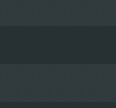
\includegraphics[width=0.5\linewidth]{Figure1.jpg}
    \caption{High-level Architecture of the System}
    \label{fig:Figure_1}
\end{figure}

\newPart{Client}

Client is directly communicate with clients. It deploys on the clients' machine and provides some APIs for clients, including 'AddCustomer', 'ReserveFlight', etc. It recieves commands from clients and proceeds them to the server (Middleware). 
After server finishing to process the commands, it recieves the execution results and prints out on the screen.

\newPart{Middleware}

Middleware is mainly consisted by four parts: RMIMiddleware, Transaction Manager, Lock Manager and Customer Remote Manager. 

1. RMIMiddleware is the only part of the server which directly communicates with Client. It exposes all APIs that Client needs and coordinates all of these commands in the server side. 

2. Transaction Manager mainly takes charge in the concurrency control of all transactions. It holds the transaction ID list and the corresponding RMs for every transaction. It also acts like the coordinator in the 2 Phase Commit.

3. Lock Manager ensures the data integrity among concurrent transactions. The system uses 2 Phase Locking algorithm and all locks of data are managed in the Lock Manager.

4. Customer RM takes charge in managing the data of the customers, including customer ID and reservations of every customer.

\newPart{Remote Managers}

There are three distributed databases deployed in three different remote machines, which are managed by three Resource Managers separately. They are Flight RM, Car RM and Room RM, which take charge in reading, writing and committing/aborting the data of flights, cars and rooms.

\newQuestion{Individual features:}

The distributed booking system has several features that insure it runs well when handling several transactions from different clients concurrently. Basically there are four main features: distribution and communication, transactions and locking (2PL), data shadowing and logging and recovery (2PC).

\newPart{Distribution and communication}

The system uses

\newPart{Transactions and locking}

We implement a centralized lock manager, letting middleware manage locks of all items. For each method a transaction calls, the middleware will first call its \textit{lockSomething} method. The transaction manager in the middleware will first check if the transaction exists. If not, a \textit{InvalidTransactionException} will be threw. Then the lock manager will try to grant a corresponding lock on that item to the transaction. If either the lock granting failed or a DeadlockException is threw, middleware will abort this transaction and throw a \textit{TransactionAbortedException}. Only the \textit{lockSomething} succeeds can the subsequent operations be executed. For example, in a \textit{reserveCar} operation, the middleware will try to grant a WRITE lock on the car and  a WRITE lock on the customer to this transaction. If both succeed, the real \textit{reserveCar} operation will be executed.

When a transaction request a lock on an item on which the transaction already has a lock, there are three situations that may happen: (1) request: read, have: read (2) request: write, have: write; (3) request: write, have: read. For (1) and (2), Lock Manager will raise RedundantLockRequestException and return true; for (3), Lock Manager will first check if other transactions are granted locks on this item. If not, Lock Manager will delete the read lock and grant a write lock to this transaction.

\newPart{Data shadowing}

\newPart{Logging and recovery (2-PC)}

\newQuestion{Special features:} We also implement the transaction manager in the middleware, but add some other data structures in the resource managers.

\textbf{Map from xid to related RMs in TransactionManager}: When Middleware reconnects to RMs after whoever crashes, we need to update the whole map if we store RM as a reference here. Instead, we only store the RM's name and add a small Hashtable which maps the name to the reference. So when reconnection happens, TransactionManager only need to update each reference one time at most.

\textbf{Crash detection:} Middleware need to detect the crash of RMs so that it can reconnect to the RM on time. We create a new Thread in which Middleware will ping the three RMs (send an empty message). Whenever this thread catches a RemoteException it knows that this RM crashed, so it will try to reconnect the RM and update the reference in TM.

\newPart{Data Structures in TransactionManager}

\newQuestion{Problems:}

\newQuestion{Testing:}

\pagebreak







1. Hashtable<Integer, Vector<IResourceManager> > xid\_rm: store active transactions and corresponding ResourceManagers on which the transaction do some operations.

2. Hashtable<Integer, Long> xid\_time: store active transactions and the start time of its last operation.

\newPart{Data Structures in ResourceManager}

1. HashMap<Integer, RMHashMap> origin\_data: store transactions that modified data of this RM and the list of original data that the transaction modified.

\newPart{Ways of Finishing Related Operations}

\textbf{Start:} When a client call Middleware's \textit{start} method, Middleware forwards it to TransactionManager TM, TM has a static variable, \textit{num\_transaction}, recording the number of transaction and return the next number as xid, which will be returned to the client. Meanwhile, TM will also add xid to its \textit{xid\_rm} and \textit{xid\_time}.

\textbf{Operations:} For each operation, Middleware will first apply a lock for this transaction by calling \textit{lockSomething}. In a \textbf{\textit{Query}} operation, Middleware will apply a READ lock on this item; in a \textbf{\textit{Add}} or \textbf{\textit{Delete}} operation, Middleware will apply a WRITE lock on this item; in a \textbf{\textit{ReserveItem}} operation, Middleware will apply a WIRTE lock on both the item and the customer. In a \textbf{\textit{DeleteCustomer}} and a \textbf{\textit{Bundle}} operation, Middleware will apply WRITE locks on the customer and all related items. Meanwhile, in all \textbf{\textit{Add, Delete, Bundle, DeleteCustomer}} operations, we need to store the original data to \textbf{origin\_data} in case abort happened. Considering all modify-related operations are finished by calling \textbf{\textit{writeData}} and \textbf{\textit{removeData}} on corresponding RMs, we add the original data to \textbf{\textit{origin\_data.get(xid)}}. If the operation creates new item, we add the original data as (key, null), in which null indicates that this is a new added item and thus need to be deleted when abort happens. 

\textbf{Abort:} Abort will happen in three situation: (1) Client call Abort; (2) DeadLock happens; (3) The transaction timed out and aborted by the transaction manager in the middleware. The only difference among them is the way that client is notified about the abort. In (1), it's no need to notify the client; in (2), client is notified by catching a TransactionAbortedException threw by the middleware; in (3), client will not be notified until it calls the next operation on this transaction and catch a InvalidTransactionException. In all three situation, the middleware will call tm.abort(xid) first, in which TM will call abort of RMs related to this transaction. Each RM will recover the data stored in \textbf{\textit{origin\_data.get(xid)}}, and reset \textbf{\textit{origin\_data.get(xid)}}. Then the middleware will also recover its own data, as a Customer-RM. At last, Lock Manager LM will release all locks of this transaction by calling \textit{unlockAll}.

\textbf{Commit:} When a client calls \textit{commit}, the Middleware forwards it to TM, and TM will commit all related RMs and delete this transaction from activeTransaction. Each RM only need to reset \textbf{\textit{origin\_data.get(xid)}}. Then the middleware will also reset its \textbf{\textit{origin\_data.get(xid)}}, as a Customer-RM. At last, Lock Manager LM will release all locks of this transaction by calling \textit{unlockAll}.

\textbf{Shutdown:} When a client calls \textit{shutdown} of the Middleware, Middleware will first call \textit{shutdown} of three RMs, and then \textit{exit()} itself. In each RM, RM will exit itself, too.

\newQuestion{4. Time-to-live Mechanism:} We implement this function by creating a new Thread in Middleware, which for-loop all active transactions and checks if System.currentTimeMillis() - xid\_time.get(xid) > MAX\_EXIST\_TIME. If so, Middleware will abort this transaction. Client will know this abortion when it calls next operation on this transaction and catch a UnvalidTransactionException. We update xid\_time.get(xid) in the middleware's \textit{lockSomething} function because each operation will call Lock first.
% \maketitle
% \tableofcontents
% 在文章类article/ctexart中定义了五个控制序列来调整行文组织:
% section\{\}
% subsection\{\}
% subsubsection\{\}
% paragraph\{\}
% subparagraph\{\}
\end{document}